\capitulo{6}{Trabajos relacionados}

\section{Lingmotif~\cite{lingmotif}}
Lingmotif es una aplicación multi-plataforma de sobremesa que analiza textos desde la perspectiva 
del Análisis de Sentimiento. \\Básicamente, es capaz de determinar la orientación semántica 
(si es positivo o negativo y en qué grado) de un texto o conjunto de textos, mediante \textbf{la detección 
de expresiones lingüísticas} que indican una determinada polaridad.

A diferencia de la mayoría del software existente, Lingmotif no es un sólo un clasificador, 
ya que no se limita a clasificar un texto como positivo o negativo, sino que además ofrece una 
serie de datos cuantitativos, una visualización del ``perfil de sentimiento'' del texto o textos 
(incluyendo series temporales), y un detallado análisis cualitativo del texto en sí, en el que 
se muestran los segmentos textuales identificados. \\Estas funcionalidades lo convierten en un herramienta 
única, y sus aplicaciones van más allá de las que normalmente ofrece este tipo de software. 
Lingmotif ofrece los resultados de sus análisis en archivos con formato HTML, con la versatilidad y 
fácil manejo que esto supone.

Actualmente Lingmotif analiza textos en español e inglés. Se está trabajando en nuevas versiones 
para alemán e italiano.

\section{Lexalytics~\cite{lexalytics}}
Lexalytics es una empresa que se especializa en tecnologías de análisis de texto y 
procesamiento del lenguaje natural (PLN).\\
Ofrece soluciones para extraer información de datos de texto no estructurados, 
como contenido de redes sociales, comentarios de clientes, reseñas y más. 
Los productos de Lexalytics están diseñados para ayudar a las empresas a analizar 
y comprender el sentimiento, los temas y las tendencias dentro de grandes volúmenes de información textual.
Uno de sus productos destacados es la Plataforma de Inteligencia Lexalytics, 
que incluye varias herramientas y funciones para el análisis de texto.
\begin{figure}[h]
    \advance\leftskip0cm 
    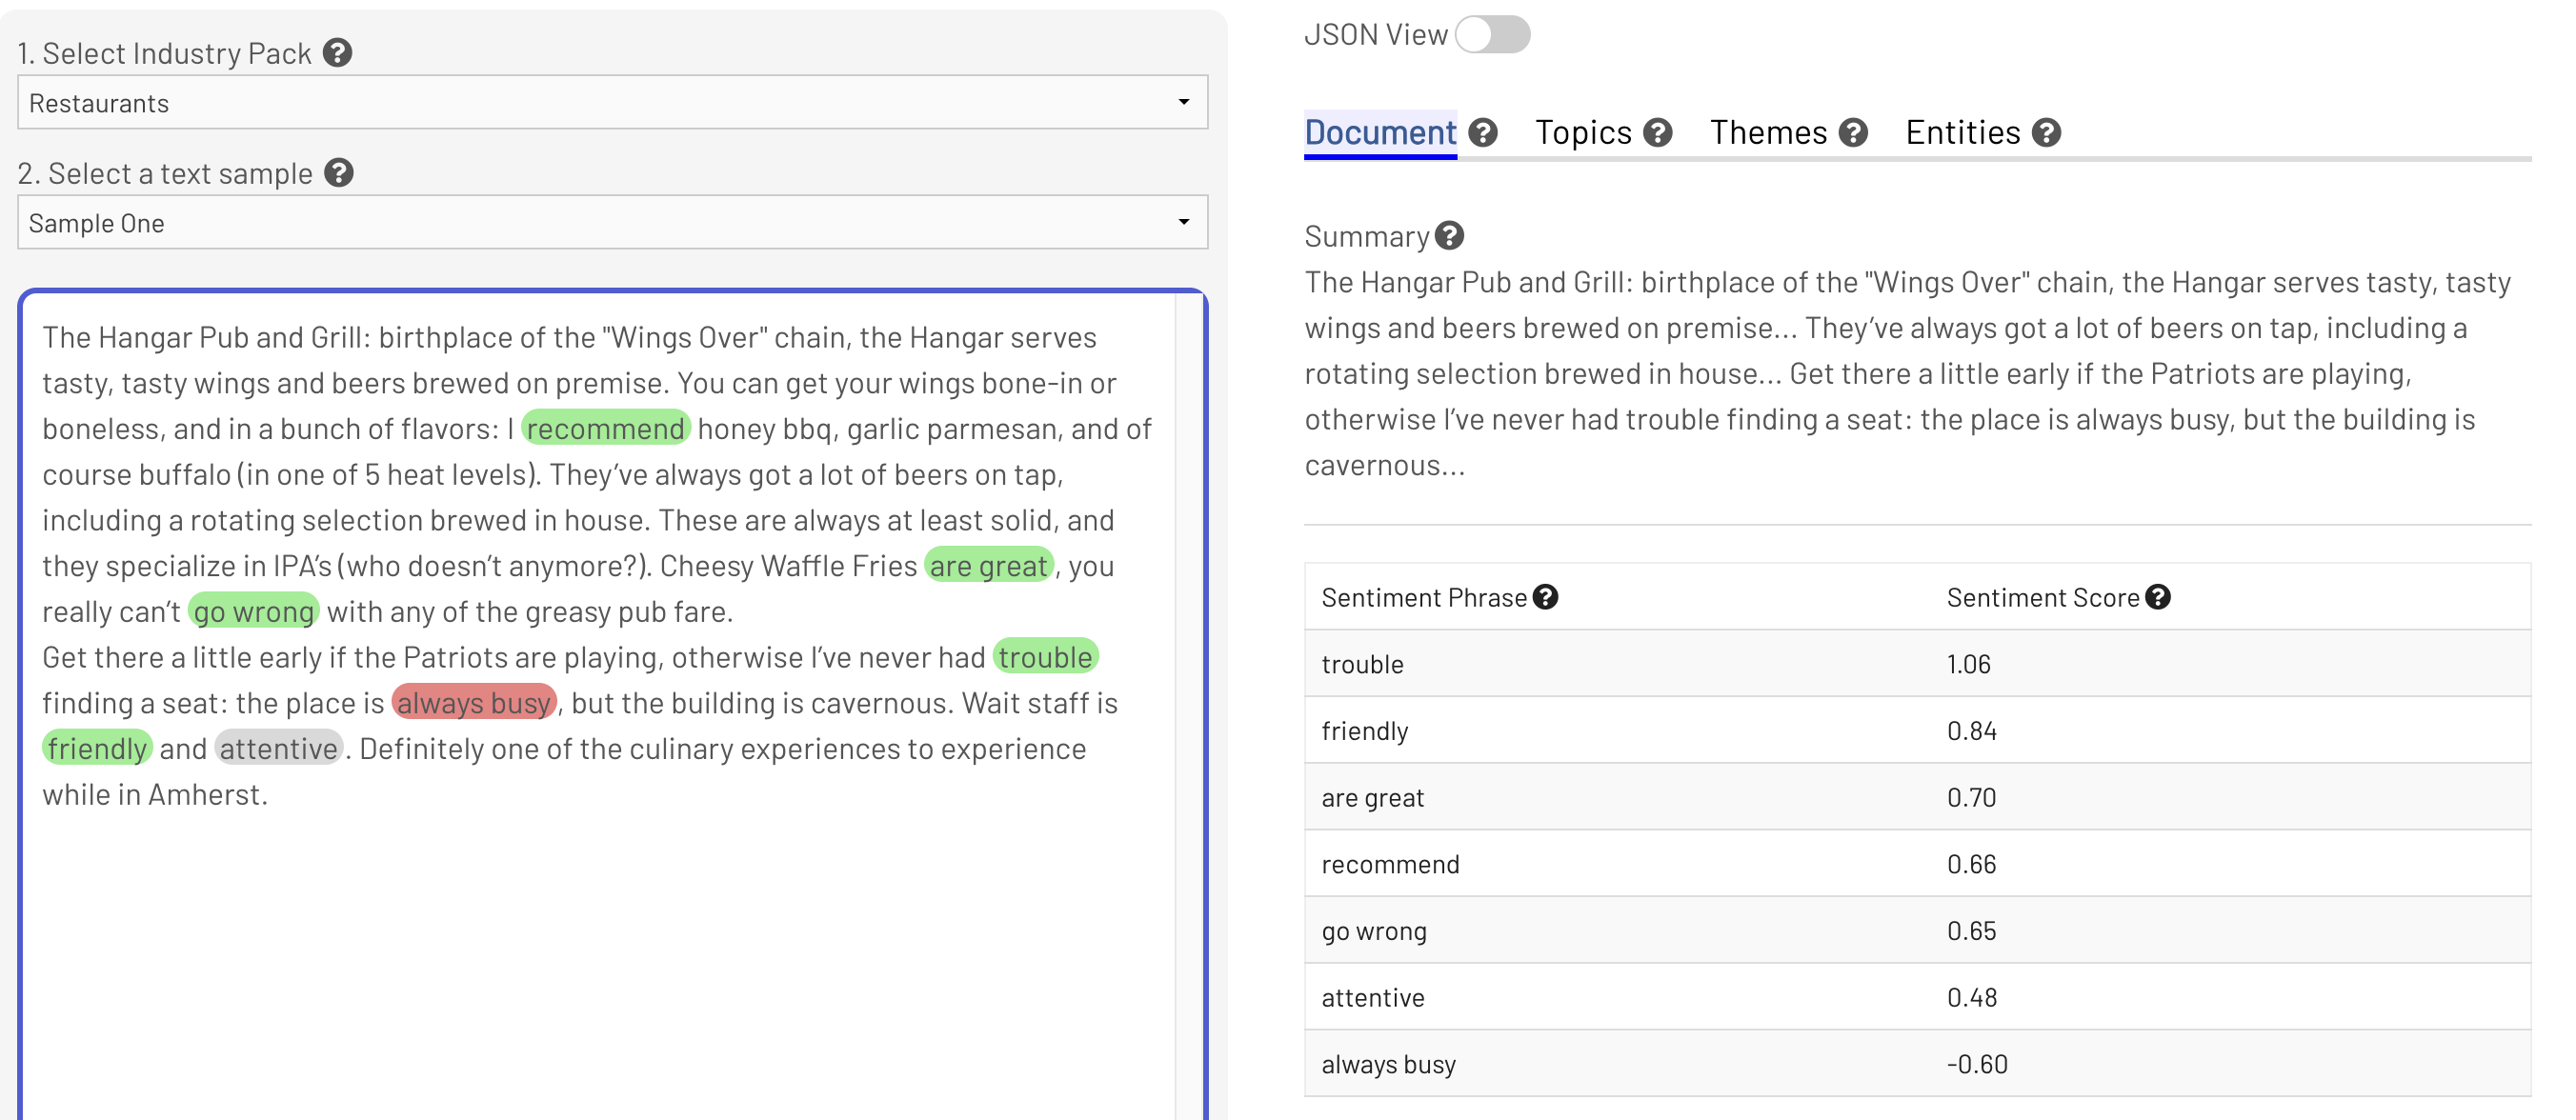
\includegraphics[scale=0.25]{lexalytics_ejemplo.png}
    \caption{Lexalytics análisis de texto}
\end{figure}
Tienen un API (llamado Semantria) que se usa para análisis de texto y sentimiento.
Admite varios idiomas, lo que las hace adecuadas para empresas con presencia global.\\
Estas herramientas y servicios pueden ser valiosos para empresas que 
buscan dar sentido a la gran cantidad de texto no estructurado que generan o 
encuentran en el curso de sus operaciones. \\Se pueden aplicar en áreas como la gestión 
de la experiencia del cliente, el monitoreo de redes sociales, la investigación de mercado 
y otros campos donde comprender la información textual es crucial.


\section{IBM Watson Studio~\cite{ibmwatson}}
IBM Watson Studio es una plataforma de inteligencia artificial (IA) desarrollada 
por IBM que proporciona servicios y herramientas para el procesamiento 
del lenguaje natural y otros. 
Lleva el nombre del fundador de IBM (Thomas J. Watson)
También utiliza técnicas de aprendizaje automático 
para extraer patrones a partir de grandes conjuntos de datos y realizar análisis predictivos.\\
Tiene capacidades para analizar y comprender imágenes y videos, lo que puede 
ser útil en aplicaciones como el reconocimiento facial y la interpretación de contenido visual.\\
Se ha utilizado en aplicaciones como juegos de preguntas y 
respuestas, demostrando su capacidad para competir y ganar contra humanos en contextos complejos.
Puede automatizar tareas y procesos empresariales, mejorando la eficiencia operativa.
Analiza datos en tiempo real para proporcionar información instantánea y tomar decisiones basadas en datos.
IBM Watson se ha aplicado en diversos campos obtenido muy buenos resultados.
Permite crear un cuenta gratuita (limitada) para poder probarla.

\section{Sentinel~\cite{Sentinel1}}
Sentinel es una aplicación web desarrollada como TFG del grado de ingeniería 
informática de la Universidad de Burgos que realiza un análisis de sentimientos de textos 
extraídos de las redes sociales Twitter e Instagram.\\
La aplicación busca los tweets relacionados con la palabra introducida 
en el caso de Twitter, o los comentarios que le han escrito a la 
cuenta de Instagram que se ha buscado.\\
Después analiza el sentimiento que hay en ellos, los puntúa con valores entre 0 y 1 y 
se almacenan los resultados.\\
Estos resultados se muestran al usuario en gráficos 
y tablas para hacer la experiencia más visual.\\ 
Además se le ofrece la opción de calcular series temporales a partir de los resultados, 
y se da una predicción de los valores futuros.

\section{Free Sentiment Analysis~\cite{freesentiment}}
Es una herramienta gratuita que permite realizar un analisis de sentimiento de cualquier 
texto escrito en Inglés. La herramienta califica el sentimiento con un número entre -100 y 100 
dependiendo del sentimiento detectado en el texto.
Sólo hay que pegar el texto en el cuadro de texto y pulsar el botón ``Analyze text''

Para su funcionamiento utiliza algoritmos de linguística computacional y minería de texto.
El modelo se ha entrenado usando el ``American National Corpus'' con lo que sólo funciona con 
textos en inglés americano y escritos después de 1990. 
No se conoce su funcionamiento interno pero por la descripción parece que ha usado un 
corpus anotado y usa las coincidencias de palabras para dar una nota al texto dependiendo 
de las palabras encontradas.